\documentclass[11pt, a4paper]{article}
\usepackage[a4paper, top=2.5cm, bottom=2.5cm, left=2cm, right=2cm]{geometry}

% --- PREAMBLE FOR PDFLATEX COMPATIBILITY ---
\usepackage[utf8]{inputenc}
\usepackage[T1]{fontenc}
\usepackage[english]{babel}

% Add because main language is not English (standard good practice)
\usepackage{enumitem}
\setlist[itemize]{label=-}

% --- PACKAGES ---
\usepackage{amsmath, amssymb}
\usepackage{graphicx} % For the visual diagram
\usepackage{fancyhdr} % For headers/footers
\usepackage{verbatim} % For sample input/output blocks
\usepackage{xcolor}   % For visual flair
\usepackage{wrapfig}
\usepackage{hyperref}
\usepackage{enumitem}
\usepackage{wrapfig} 


% Define \problemname and \illustration if not using Kattis template
\newcommand{\problemname}[1]{\section*{#1}}
% Updated \illustration command using wrapfigure
% #1 = width fraction (e.g., 0.3)
% #2 = image filename
% #3 = caption
\newcommand{\illustration}[3]{%
    \begin{wrapfigure}{r}{#1\textwidth} % 'r' places it on the right
        \centering
        \vspace{-10pt}
        \includegraphics[trim={0cm 10cm 0 10cm},clip, width=\linewidth]{#2}
        \vspace{-25pt}
        \caption{#3}
        \vspace{-20pt} % Removes excess whitespace below caption
    \end{wrapfigure}
}

\begin{document}


\problemname{The Scenic Route}

% This command now places the image on the right, allowing text to wrap on the left
\illustration{0.45}{Images/Trans_Canada_Highway.png}{Photo by \href{https://www.nationalgeographic.com/travel/article/ultimate-trans-canadian-highway-roadtrip}{National Geographic}}

You just got engaged and are planning the ultimate scenic road trip across Canada. You plan on taking the Trans-Canada Highway, Canada's longest national road, stretching from Victoria, BC to British Columbia, and ending in St. John's, Newfoundland and Labrador. It was once the world's longest uninterrupted highway when it opened in 1962. We represent the highway as a straight line with $N$ distinct sections, \mbox{indexed from ~$1$ to ~$N$.}\\

\noindent Initially, the highway is boring, with a "Scenic Value" of $0$ for each section. However, before the tourist season begins, the Department of Transportation completes a series of $M$ beautification projects. Each project targets a specific contiguous range of the highway $[L, R]$ and increases the Scenic Value of every section in that range by an integer $V$.\\

\noindent Once the Department finishes these projects, the highway is ready for travel. You start to plan your road trip, but you encounter an issue... \\

\noindent Unfortunately, because of the new beautification projects, an increased number of people have started driving on the highway. Due to this influx in traffic, accidents may occur at specific sections of the highway. An accident acts as a complete roadblock. You cannot drive through a section that has an accident, nor can you start or end your trip there. (You must start your trip at the next section or end it at the section before the accident)\\

\vspace{10pt}
\noindent \textbf{The Trip Rule:}
You must choose a single contiguous segment of the highway to drive on. This segment must not contain any accidents. Your goal is to maximize the \textbf{Total Scenic Value} (the sum of values of all sections) of your trip.\\

\noindent The input provides the details of the beautification projects, followed by $Q$ different traffic scenarios. For each scenario, you must calculate the maximum Total Scenic Value possible.

% --- DIAGRAM PLACEHOLDER ---
\begin{figure}[h]
    \centering
    \framebox{
        \parbox{0.9\textwidth}{
            \centering
            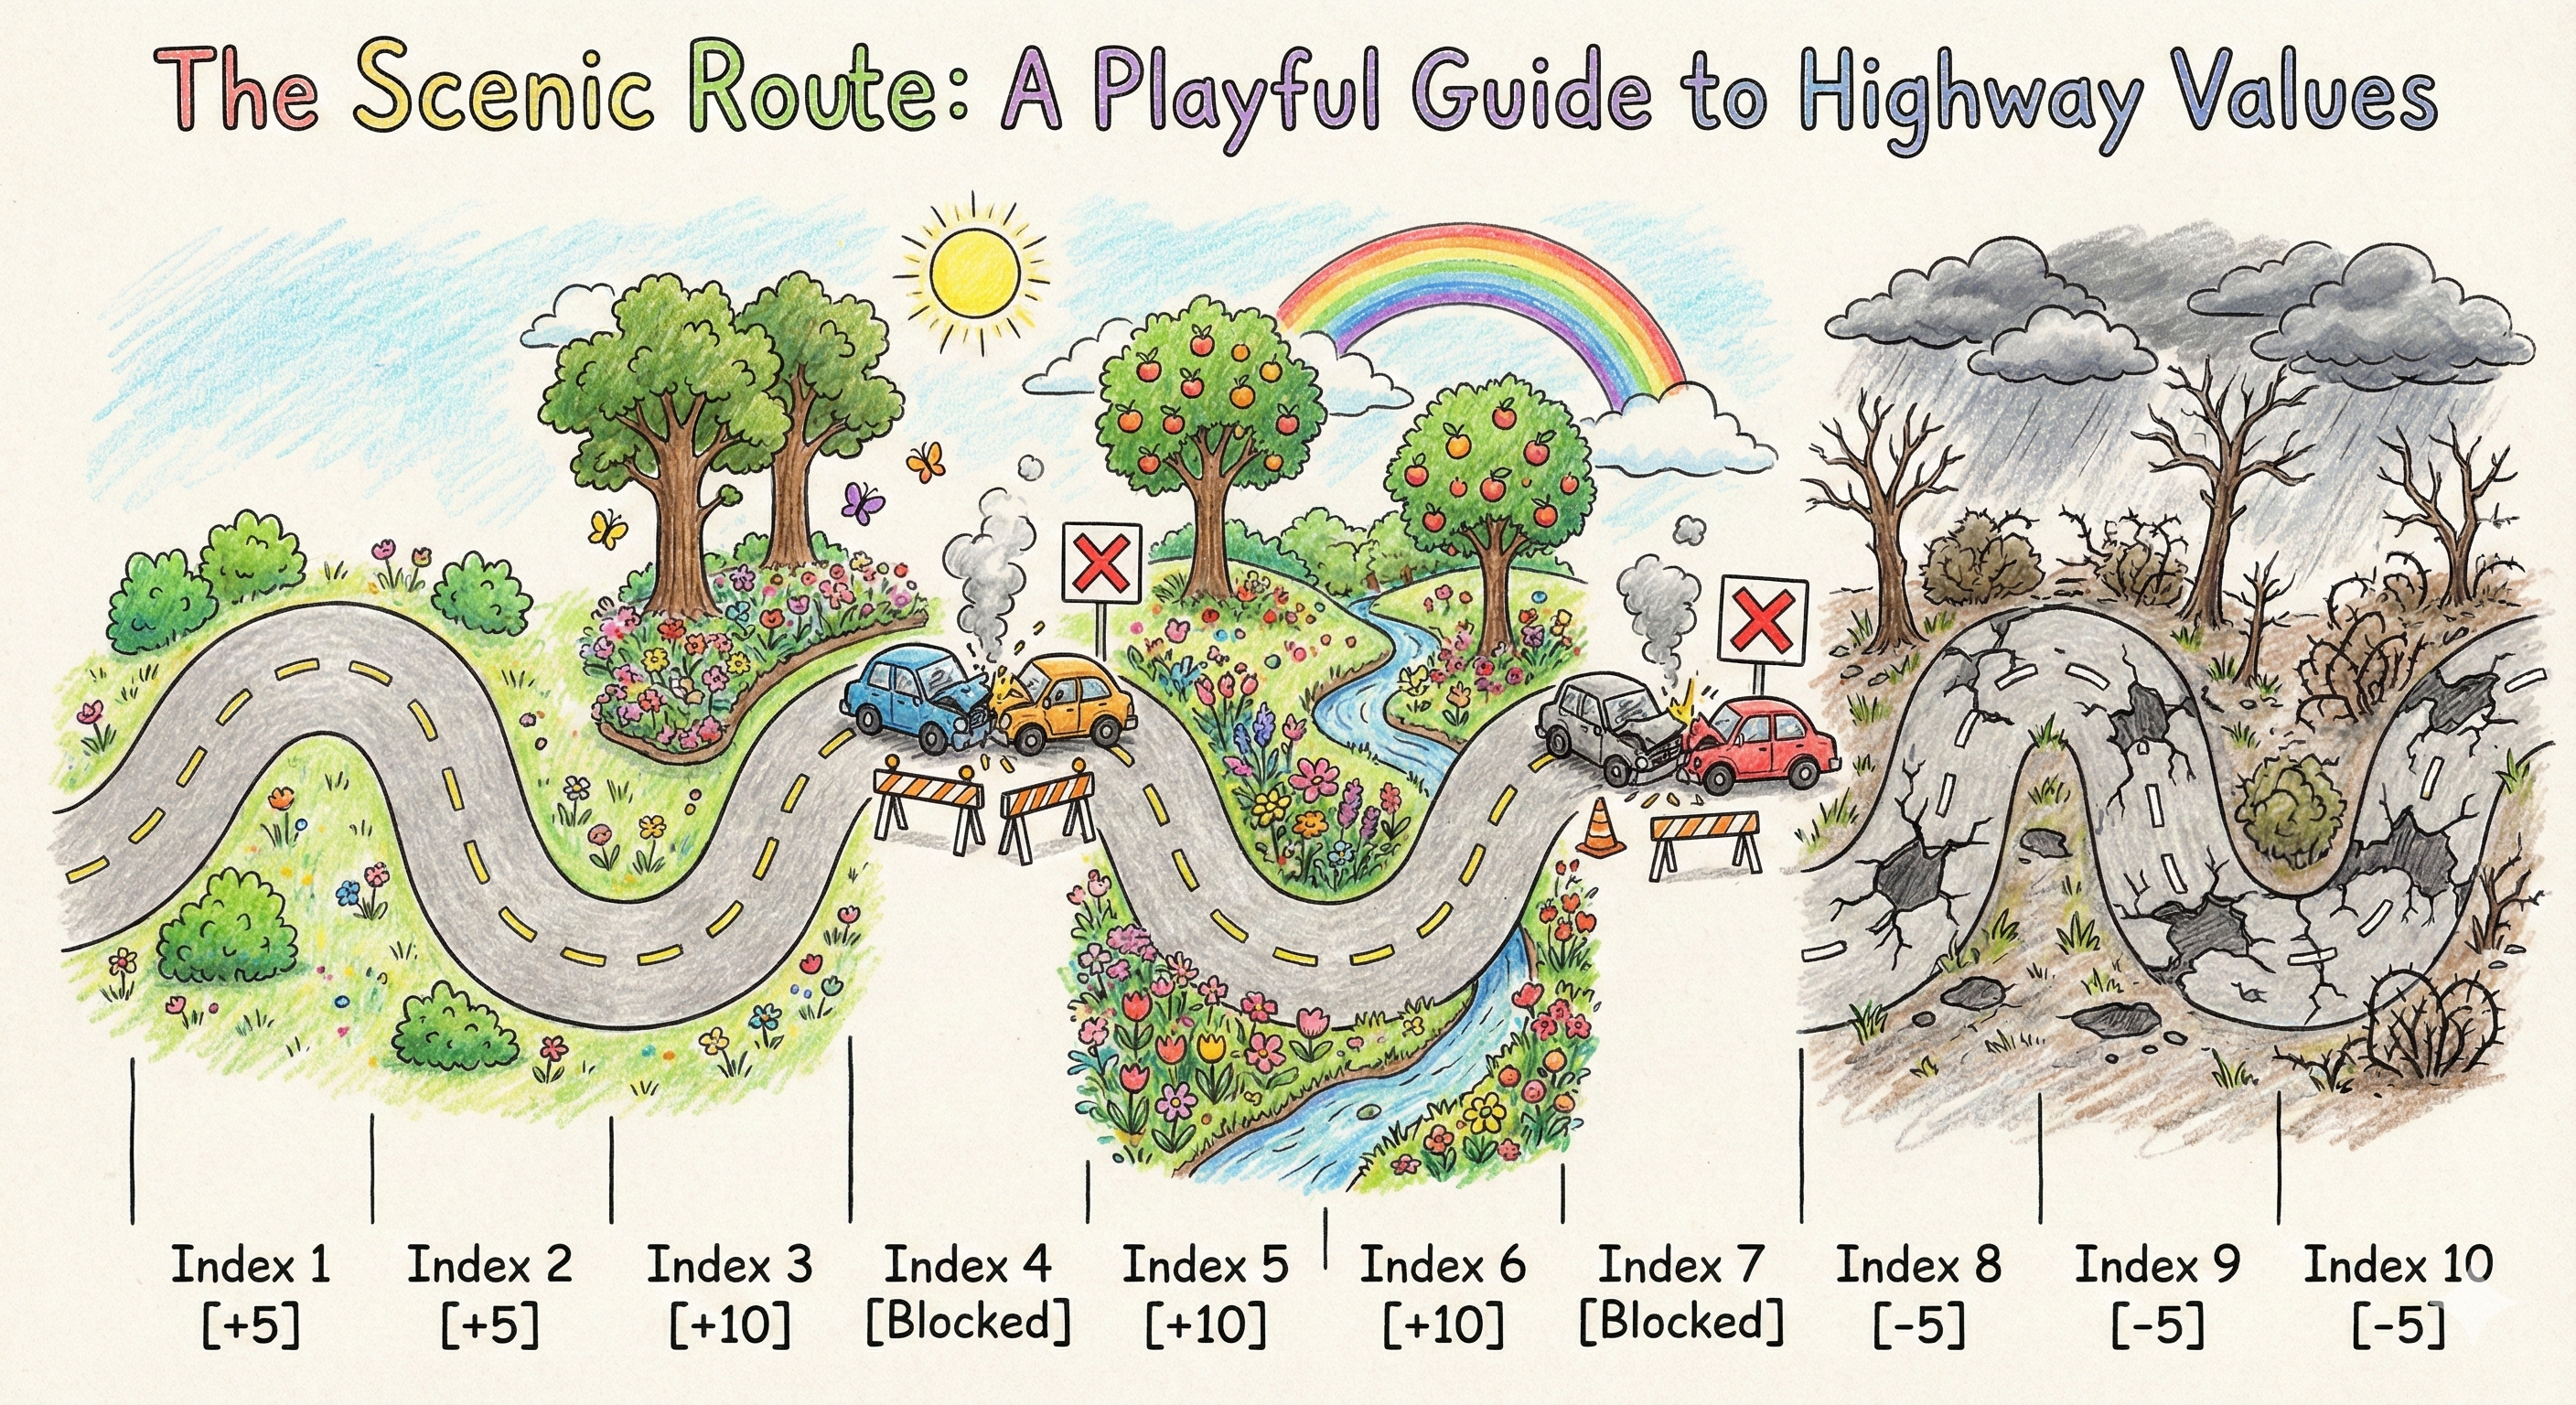
\includegraphics[trim={0cm 0cm 0 7cm},clip, width=0.8\textwidth]{Images/Visual Representation.png}\\
            In this example, an accident at index 4 and 7 splits the road into three drivable segments: \\
            Indices $[1, 3]$, Index $[5, 6]$, and Index $[8, 8]$.
        }
    }
    \caption{An accident at section $i$ forces you to choose a segment entirely before $i$ or entirely after $i$.}
\end{figure}

\newpage
\section*{Input}

The first line contains two integers $N$ and $M$ ($1 \le N, M \le 200\,000$), representing the length of the highway and the number of beautification projects. \\

\noindent The next $M$ lines describe the projects. Each line contains three integers $L, R, V$:
\begin{itemize}
    \item The range $[L, R]$ ($1 \le L \le R \le N$) has its Scenic Value increased by $V$ ($-1000 \le V \le 1000$).
\end{itemize}
\textit{Note: $[L, R]$ is inclusive. A negative $V$ represents construction work that makes the scenery ugly.}\\

\noindent The next line contains an integer $Q$ ($1 \le Q \le 20\,000$), the number of traffic scenarios to analyze.

\noindent For each of the $Q$ scenarios:
\begin{itemize}
    \item The line contains $K$ distinct integers $a_1, a_2, \dots, a_K$ ($1 \le a_i \le 10$), representing the locations of the accidents.
\end{itemize}


% --- OUTPUT ---
\section*{Output}

For each of the $Q$ scenarios, output a single integer on a new line: the maximum Total Scenic Value obtainable on a single valid continuous drive. \\ 

\noindent If the best possible drive has a negative total value, you may still drive (output the negative sum). If each section is blocked, output \verb|impossible|.

\section*{Sample Input 1	Sample Output 1}

\vspace{10pt}
\noindent \textbf{\large Sample Input 1}
\begin{verbatim}
10 3
1 10 5
3 7 5
8 10 -10
3
4 7 
5
1 2 3 4 5 6 7 8 9 10
\end{verbatim}

\vspace{10pt}
\noindent \textbf{\large Sample Output 1}
\begin{verbatim}
20
30
Impossible
\end{verbatim}

\newpage

\noindent \textbf{Explanation of Sample 1:}
\begin{itemize}
    \item \textbf{Step 1 (Highway Beautification):}
    \item Initially: $[0, 0, 0, 0, 0, 0, 0, 0, 0, 0]$
    \item Update 1 (1-10, +5): $[5, 5, 5, 5, 5, 5, 5, 5, 5, 5]$
    \item Update 2 (3-7, +5): $[5, 5, 10, 10, 10, 10, 10, 5, 5, 5]$
    \item Update 3 (8-10, -10): $[5, 5, 10, 10, 10, 10, 10, -5, -5, -5]$
    \item \textbf{Final Values:} $[5, 5, 10, 10, 10, 10, 10, -5, -5, -5]$\\
    
    \item \textbf{Scenario 1:} Accidents at $\{4, 7\}$.
    \item Blocked indices: 4 and 7.
    %[ 5 | 5 | 10 | 10 | 10 | 10 | 10 | -5 | -5 | -5 ]
    \item Highway: [ 5 | 5 | 10 | \textbf{X} | 10 | 10 | \textbf{X} | -5 | -5 | -5 ]

    \item Available Segments: $[1, 3]$, $[5, 6]$, $[8, 10]$.
    \item Sum $[1, 3] = 5+5+10 = 20$.
    \item Sum $[5, 6] = 10+10 = 20$.
    \item Sum $[8, 10] = -5 + -5 + -5 = -15$.
    \item Max is \textbf{20}
    \item Output: \textbf{20} \\

    \item \textbf{Scenario 2:} Accidents at $\{5\}$.
    \item Blocked indices: 5.    
    \item Highway: [ 5 | 5 | 10 | 10 | \textbf{X} | 10 | 10 | -5 | -5 | -5 ]
    \item Available Segments: $[1, 4]$, $[6, 10]$
    \item Sum $[1, 4] = 5+5+10+10 = 30$.
    \item Sum $[6, 10] = 10+10-5-5-5 = 5$.
    \item Max is \textbf{30}
    \item Output: \textbf{30} \\

    \item \textbf{Scenario 3:} Accidents at $\{1, 2, 3, 4, 5, 6, 7, 8, 9, 10\}$.
    \item Blocked indices: 1, 2, 3, 4, 5, 6, 7, 8, 9, 10.
    \item Highway: [ \textbf{X} | \textbf{X} | \textbf{X} | \textbf{X} | \textbf{X} | \textbf{X} | \textbf{X} | \textbf{X} | \textbf{X} | \textbf{X} ]
    \item Available Segments: $None$
    \item Output: \verb|Impossible|
\end{itemize}


\end{document}